\section{Desarrollo}

El desarrollo del frontend se organizó en seis fases progresivas, donde cada una 
deja las condiciones preparadas para que la siguiente pueda avanzar sin fricciones. 
Esta estrategia permitió mantener en todo momento una aplicación funcional y 
coherente, evitando estados intermedios rotos o incompletos.

% -------------------------------------------------------
\subsection{Fase 1: Módulo de Usuarios y Autenticación}

La primera fase establece las bases del sistema desde la perspectiva del usuario 
final: el acceso a la aplicación y la navegación según el rol asignado.

\subsubsection*{Layouts}

Se definen dos layouts que encapsulan la estructura visual de las rutas de la 
aplicación. \texttt{AuthLayout} es el layout público, utilizado exclusivamente por 
\texttt{/login}; centra el contenido sobre un fondo degradado oscuro y no incluye 
ningún elemento de navegación, como se aprecia en la figura~\ref{fig:01_auth_layout}.
\texttt{AppLayout} es el layout principal para todas 
las rutas privadas; integra \texttt{AppSidebar} y \texttt{AppTopbar} como componentes 
de navegación persistentes, mientras que el contenido de cada ruta se renderiza 
dentro de \texttt{<RouterView />}. La separación entre ambos layouts permite que la 
pantalla de login sea completamente independiente del shell de la aplicación, sin 
necesidad de condicionar su visibilidad desde un único componente raíz.

\subsubsection*{LoginView y flujo de autenticación}

\texttt{LoginView} recibe las credenciales del usuario y delega en el servicio 
\texttt{auth.service} para realizar el \texttt{POST /auth/login}. Ante una respuesta 
exitosa, el token JWT se persiste en \texttt{localStorage} a través de 
\texttt{useAuthStore}, y los datos del usuario autenticado se cargan inmediatamente 
mediante \texttt{getMyUser()} y se almacenan en \texttt{useUserStore}. Si el usuario 
provino de una ruta protegida, el router lo redirige al destino original; en caso 
contrario, a \texttt{HomeView}, cuya vista se puede apreciar en las 
figuras~\ref{fig:02_homeview_admin} y~\ref{fig:03_homeview_user}.
Los errores de credenciales (\texttt{401}) y de 
cuenta inactiva (\texttt{403}) se muestran como mensajes descriptivos en la misma 
vista, sin requerir componentes externos.

\subsubsection*{Control de acceso y guards de navegación}

El control de acceso se implementa en \texttt{router/index.ts} mediante un guard 
global ejecutado en \texttt{beforeEach}. Las rutas privadas llevan la meta 
\texttt{requiresAuth: true}; las rutas exclusivas de administrador llevan además 
\texttt{requiresAdmin: true}. El guard consulta \texttt{useAuthStore} para verificar 
autenticación y \texttt{useUserStore} para verificar el rol de administrador, 
redirigiendo al login o al home según corresponda. Esto garantiza que un usuario con 
\texttt{is\_admin = false} solo pueda acceder a \texttt{HomeView}, 
\texttt{DeviceCatalogView}, \texttt{MyLoansView} y \texttt{MyUserView}.
Dentro de las figuras~\ref{fig:02_homeview_admin} y~\ref{fig:03_homeview_user} 
se aprecia el control de acceso diferenciado para cada tipo de usuario.

\subsubsection*{Vistas de usuario}

\texttt{UsersListView} es la vista de administración de usuarios, accesible solo bajo 
\texttt{/admin/users}; permite listar, crear, editar y eliminar usuarios, y gestionar 
sus roles mediante el repositorio de \texttt{roles}, como se aprecia en la 
figura~\ref{fig:04_users_list_view}.
\texttt{MyUserView} expone los 
datos del usuario autenticado obtenidos desde \texttt{GET /users/me}, permitiendo 
consultar su perfil sin necesidad de conocer su identificador numérico, como se 
aprecia en la figura~\ref{fig:05_my_user_view}.

% -------------------------------------------------------
\subsection{Fase 2: Módulo de Catálogo}

La segunda fase implementa la gestión del catálogo de referencia, exclusiva para 
administradores.

\texttt{CatalogView}, disponible en \texttt{/admin/catalog}, agrupa en una sola 
vista la administración de \texttt{brands}, \texttt{models}, \texttt{categories}, 
\texttt{statuses} y \texttt{ubications}, algunas de cuyas secciones se pueden 
apreciar en las figuras~\ref{fig:06_catalog_roles}, \ref{fig:07_catalog_ubicaciones}, 
\ref{fig:08_catalog_estados} y~\ref{fig:09_catalog_modelos}.
Cada entidad se presenta en una sección 
con su propia tabla y formulario de creación y edición. Las operaciones disponibles 
son listado, creación, edición y eliminación, todas consumiendo los endpoints del 
módulo de catálogo del backend.

Una consideración importante respecto a \texttt{statuses}
(ver figura~\ref{fig:08_catalog_estados}):
los estados del sistema 
son estáticos e imborrables desde la interfaz. Esto se debe a que su uso es único y 
vital para el funcionamiento del ciclo de vida de los préstamos y del historial de 
dispositivos: nombres como \texttt{`disponible'}, \texttt{`pendiente'}, 
\texttt{`aprobado'}, \texttt{`rechazado'}, \texttt{`prestado'} y 
\texttt{`devuelto'} son referenciados por nombre directamente en la lógica del 
repositorio del backend. Eliminar o renombrar un estado desde el frontend 
comprometería el funcionamiento de todo el sistema, por lo que la vista solo permite 
su visualización, sin exponer botones de edición ni eliminación para esta entidad.

% -------------------------------------------------------
\subsection{Fase 3: Módulo de Productos}

La tercera fase introduce la primera vista con distinción explícita de roles dentro 
del mismo recurso.

\texttt{ProductsListView}, accesible en \texttt{/admin/products}, permite al 
administrador crear, editar y eliminar productos. Cada producto puede vincularse 
opcionalmente a entidades del catálogo: marca, modelo y categoría. 
\texttt{ProductDetailView}, accesible en \texttt{/admin/products/:id}, expone el 
detalle completo de un producto junto con los dispositivos asociados a él.
Las vistas implementadas para \texttt{ProductsListView} se pueden apreciar en las 
figuras~\ref{fig:10_products_list_admin}, \ref{fig:11_products_list_nuevo} 
y~\ref{fig:12_products_list_detalles}.

Es a partir de esta fase donde comienza a evidenciarse en el frontend la necesidad 
de las eliminaciones en cascada en la base de datos. Al implementar la eliminación 
de un producto desde la interfaz, se detectó que los dispositivos asociados a dicho 
producto no se eliminaban correctamente, dejando registros huérfanos. Esto requirió 
la corrección de la relación \texttt{ON DELETE CASCADE} entre \texttt{devices} y 
\texttt{products}, gestionada mediante Alembic tal como se describe en la sección 
\ref{sec:alembic_uso}. Esta fase dejó los productos con su estructura de datos 
completa y sus relaciones con el catálogo correctamente establecidas, listos para 
ser consumidos por el módulo de dispositivos en la fase siguiente.

% -------------------------------------------------------
\subsection{Fase 4: Módulo de Dispositivos}

La cuarta fase implementa la gestión de las unidades físicas del inventario y 
habilita la interacción del usuario común con el catálogo de dispositivos 
disponibles.

\texttt{DevicesListView}, accesible en \texttt{/admin/devices}, permite al 
administrador registrar nuevos dispositivos, editarlos, cambiar su estado y 
eliminarlos. Cada dispositivo se vincula a un producto y, opcionalmente, a una 
ubicación del catálogo, como se aprecia en las 
figuras~\ref{fig:13_devices_list_view} y~\ref{fig:14_devices_list_agregar}.
Al igual que en la fase anterior, la eliminación de un 
dispositivo requirió la corrección de la relación \texttt{ON DELETE CASCADE} entre 
\texttt{loan\_request\_items} y \texttt{devices}, también gestionada con Alembic 
según lo descrito en la sección~\ref{sec:alembic_uso}.
Adicionalmente, la figura~\ref{fig:15_products_filtro_devices} ilustra la integración 
de un botón dentro de \texttt{ProductsListView} que permite agregar dispositivos 
directamente desde la vista, realizando un envío hacia \texttt{DevicesListView} con 
el filtro del producto seleccionado aplicado.

\texttt{DeviceCatalogView}, accesible en \texttt{/catalog} para todos los usuarios 
autenticados, es la vista principal de interacción para el usuario común. Muestra 
únicamente los dispositivos con estado \texttt{"disponible"}, consumiendo el endpoint 
\texttt{GET /devices/available}. La vista incluye filtros por categoría y búsqueda 
por texto, y permite seleccionar uno o más dispositivos mediante casillas de 
verificación, como se aprecia en la figura~\ref{fig:16_device_catalog_view}.
Al confirmar la selección, se abre un diálogo donde el usuario puede 
ingresar un motivo y una fecha estimada de devolución, dejando todo listo para enviar 
la solicitud de préstamo, como se muestra en la figura~\ref{fig:17_device_catalog_prestamo}.
La lógica de creación del préstamo, sin embargo, no se 
activa en esta fase: los formularios y la selección quedan preparados para ser 
conectados al módulo de préstamos en la fase siguiente. Adicionalmente, la vista 
verifica solicitudes activas del usuario antes de abrir el diálogo, evitando 
solicitudes duplicadas para un mismo dispositivo.

% -------------------------------------------------------
\subsection{Fase 5: Módulo de Préstamos}

La quinta fase conecta toda la lógica preparada en fases anteriores para implementar 
el ciclo de vida completo de los préstamos.

\subsubsection*{Ciclo de vida de un préstamo}

Un préstamo atraviesa un conjunto ordenado de estados desde su creación hasta su 
cierre. El diagrama siguiente ilustra este ciclo, incluyendo el camino nominal y la 
rama de rechazo:

\begin{figure}[H]
	\centering
	\begin{tikzpicture}[
		node distance=1.6cm and 2.2cm,
		every node/.style={font=\small},
		state/.style={
			rounded corners=6pt,
			draw,
			thick,
			minimum width=2.8cm,
			minimum height=0.9cm,
			align=center,
			text width=2.6cm,
		},
		pending/.style={state, fill=yellow!25, draw=yellow!60!black},
		approved/.style={state, fill=blue!20, draw=blue!50!black},
		rejected/.style={state, fill=red!20, draw=red!60!black},
		borrowed/.style={state, fill=orange!25, draw=orange!60!black},
		returned/.style={state, fill=green!25, draw=green!50!black},
		arrow/.style={-{Stealth[length=6pt]}, thick},
		]
		
		\node[pending]  (pendiente) {pendiente};
		\node[approved] (aprobado)  [below=of pendiente]  {aprobado};
		\node[rejected] (rechazado) [right=of aprobado]   {rechazado};
		\node[borrowed] (prestado)  [below=of aprobado]   {prestado};
		\node[returned] (devuelto)  [below=of prestado]   {devuelto};
		
		\draw[arrow] (pendiente) -- node[left, font=\footnotesize]{aprobar} (aprobado);
		\draw[arrow] (pendiente) -- node[above, font=\footnotesize]{rechazar} (rechazado);
		\draw[arrow] (aprobado)  -- node[left, font=\footnotesize]{entregar} (prestado);
		\draw[arrow] (prestado)  -- node[left, font=\footnotesize]{devolver}  (devuelto);
		
	\end{tikzpicture}
	\caption{Ciclo de vida de una solicitud de préstamo en LabDIC.}
	\label{fig:ciclo_prestamo}
\end{figure}

Cada transición corresponde a una acción exclusiva del administrador y es 
irreversible: una solicitud aprobada no puede volver a estado pendiente, ni una 
solicitud rechazada puede retomarse. Los colores reflejan la semántica del estado: 
amarillo para pendiente (en espera de decisión), azul para aprobado (autorizado pero 
no entregado), rojo para rechazado (ciclo cerrado sin entrega), naranja para prestado 
(dispositivos en posesión del usuario) y verde para devuelto (ciclo cerrado 
exitosamente).

\subsubsection*{Vistas implementadas}

\texttt{AdminLoansView}, accesible en \texttt{/admin/loans}, permite al administrador 
visualizar todas las solicitudes del sistema en una tabla con \texttt{LoanStatusBadge} 
para identificar rápidamente el estado de cada una. Al seleccionar una solicitud se 
abre un \texttt{Drawer} lateral con el detalle completo: datos del solicitante, 
fechas del ciclo, dispositivos involucrados y un timeline visual del ciclo de vida. 
Desde este mismo drawer el administrador puede ejecutar las acciones disponibles 
según el estado actual: aprobar o rechazar si está pendiente, registrar entrega si 
está aprobada, y registrar devolución si está prestada. Las vistas de 
\texttt{AdminLoansView} se aprecian en las 
figuras~\ref{fig:18_admin_loans_view}, \ref{fig:19_admin_loans_ciclo_inicial} 
y~\ref{fig:20_admin_loans_ciclo_finalizado}.

\texttt{MyLoansView}, accesible en \texttt{/my-loans} para todos los usuarios 
autenticados, muestra las solicitudes propias del usuario con el mismo componente de 
timeline, permitiendo hacer seguimiento del estado de cada préstamo sin necesidad de 
contactar al administrador, como se aprecia en las 
figuras~\ref{fig:21_my_loans_view} y~\ref{fig:22_my_loans_detalles}.

% -------------------------------------------------------
\subsection{Fase 6: UX, UI y evidencias}

\subsubsection*{Revisión de experiencia de usuario}

Una vez implementadas todas las funcionalidades del sistema, se realizó una revisión 
iterativa de la experiencia de usuario desde la perspectiva del desarrollador como 
usuario de prueba. Este proceso consistió en recorrer todos los flujos de la 
aplicación, tanto desde el rol de usuario común como desde el rol de administrador, 
con el objetivo de identificar inconsistencias visuales, comportamientos inesperados 
y oportunidades de mejora que no son evidentes durante la implementación técnica.

Entre los ajustes realizados se incluyen: refinamiento de colores en los 
\texttt{LoanStatusBadge} y \texttt{DeviceStatusBadge} para mejorar la legibilidad 
según el estado; ajuste de fondos y tipografías para mantener coherencia visual entre 
modo claro y modo oscuro, ambos soportados de forma nativa a través del sistema de 
temas de PrimeVue y TailwindCSS; incorporación de mensajes \texttt{Toast} en 
operaciones críticas (creación, edición, eliminación, errores de red, sesión expirada, 
solicitudes duplicadas) para dar retroalimentación inmediata al usuario sin 
interrumpir el flujo de navegación; y validaciones visuales en formularios para 
prevenir el envío de datos incompletos o inválidos.

Adicionalmente, \texttt{HomeView} fue enriquecida con métricas simples que ofrecen 
al usuario una visión inmediata del estado del sistema al iniciar sesión. Según el 
rol del usuario autenticado, la vista muestra tarjetas de resumen con información 
relevante —como el número de dispositivos disponibles, solicitudes activas o 
préstamos pendientes de gestión— cada una con acceso directo a su vista 
correspondiente. Esto reduce la necesidad de navegar manualmente por el menú para 
obtener un panorama general, mejorando la eficiencia del flujo de trabajo tanto para 
administradores como para usuarios comunes, como se aprecia en las 
figuras~\ref{fig:02_homeview_admin} y~\ref{fig:03_homeview_user}.

La adaptación \textit{responsive} se verificó probando la aplicación en distintos 
tamaños de ventana, en orientación horizontal y vertical, y en diferentes navegadores 
(Firefox, Chrome y Edge). El layout basado en \texttt{AppSidebar} colapsable y el 
uso de componentes de PrimeVue con soporte nativo para pantallas pequeñas permitió 
que la interfaz se adapte de forma satisfactoria tanto a resoluciones de escritorio 
como a resolución adaptada a dispositivos móviles con el modo de orientación vertical 
en los navegadores de escritorio.

\subsubsection*{Evidencias de la implementación}

% [Sección reservada para capturas de pantalla y evidencias visuales de la 
%  implementación del frontend.]
\begin{figure}[H]
	\centering
	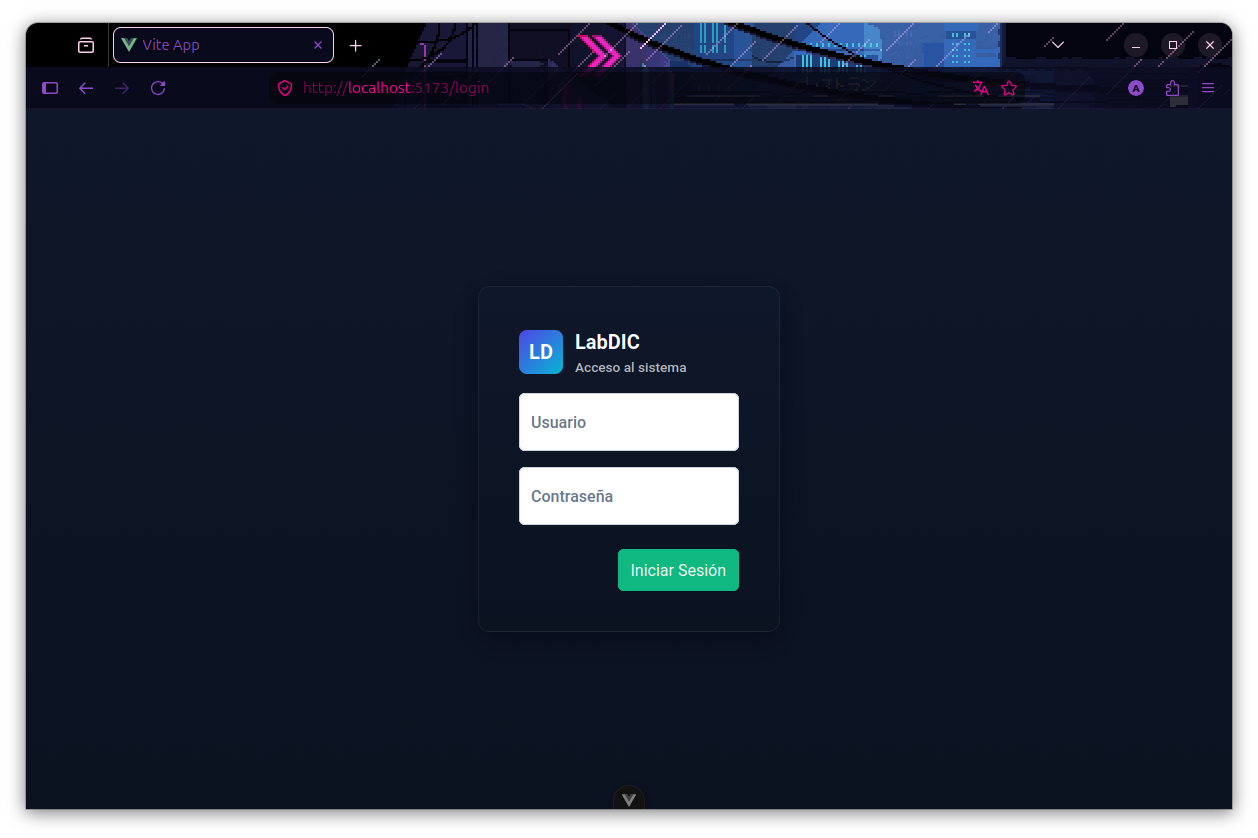
\includegraphics[width=1\textwidth]{img/01_auth_layout.png}
	\caption{Vista de autenticación — pantalla de inicio de sesión}
	\label{fig:01_auth_layout}
\end{figure}
\begin{figure}[H]
	\centering
	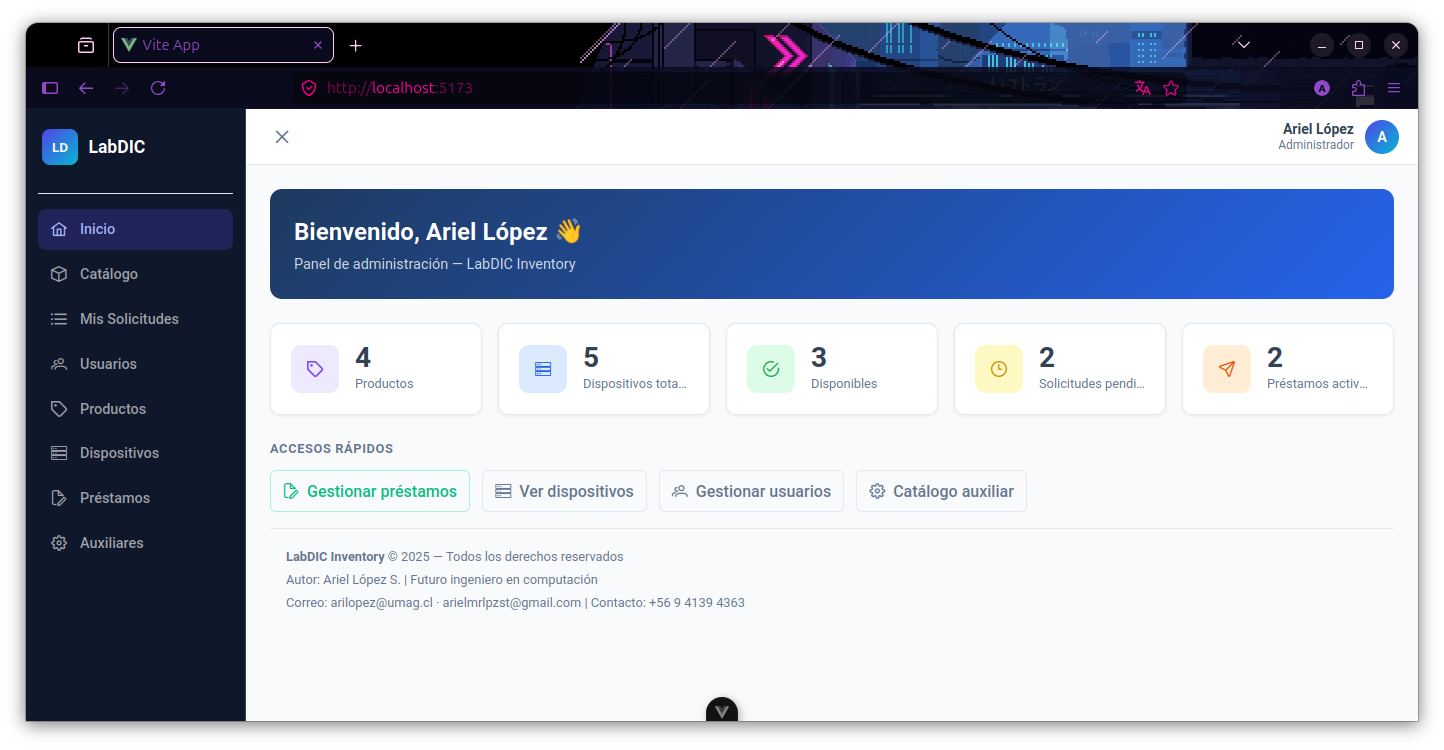
\includegraphics[width=1\textwidth]{img/02_homeView_admin_UX_UI.png}
	\caption{Vista de inicio para el rol administrador}
	\label{fig:02_homeview_admin}
\end{figure}
\begin{figure}[H]
	\centering
	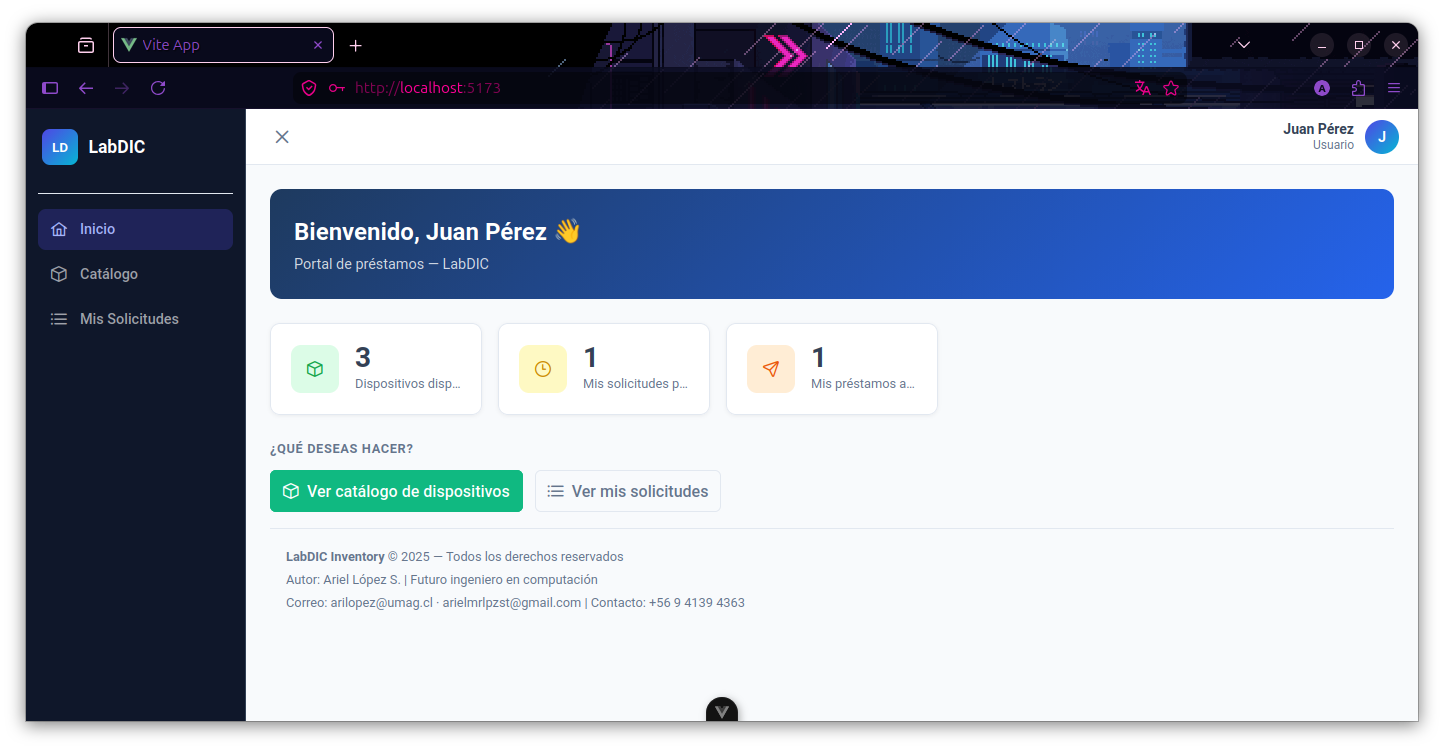
\includegraphics[width=1\textwidth]{img/03_homeView_user_UX_UI.png}
	\caption{Vista de inicio para el rol usuario}
	\label{fig:03_homeview_user}
\end{figure}
\begin{figure}[H]
	\centering
	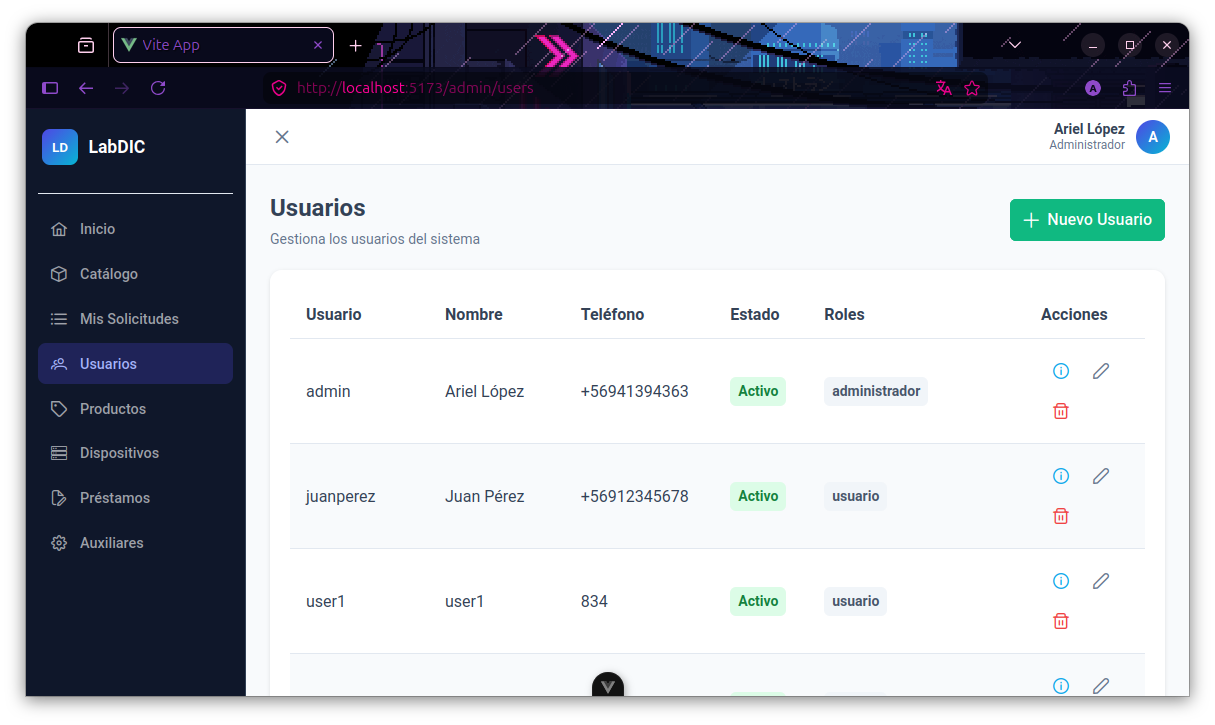
\includegraphics[width=1\textwidth]{img/04_UserListView.png}
	\caption{Vista de administración de usuarios}
	\label{fig:04_users_list_view}
\end{figure}
\begin{figure}[H]
	\centering
	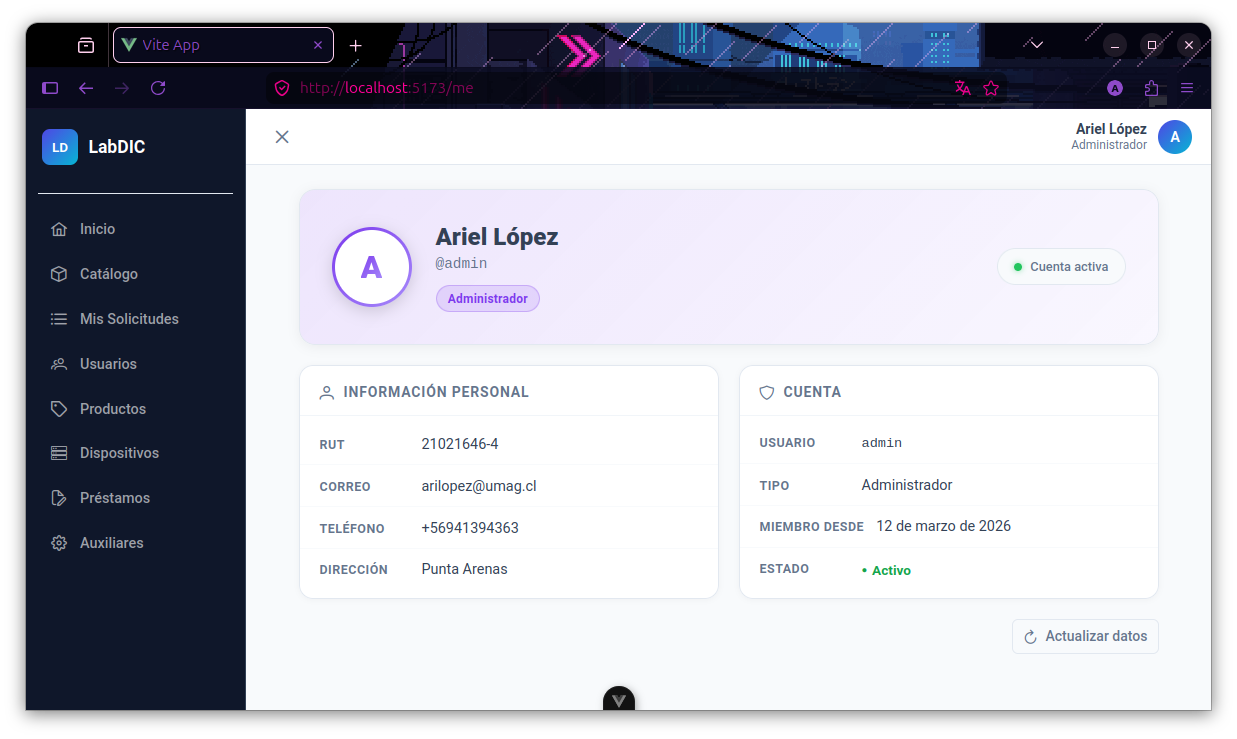
\includegraphics[width=1\textwidth]{img/05_MyUserView.png}
	\caption{Vista de perfil del usuario autenticado}
	\label{fig:05_my_user_view}
\end{figure}
\begin{figure}[H]
	\centering
	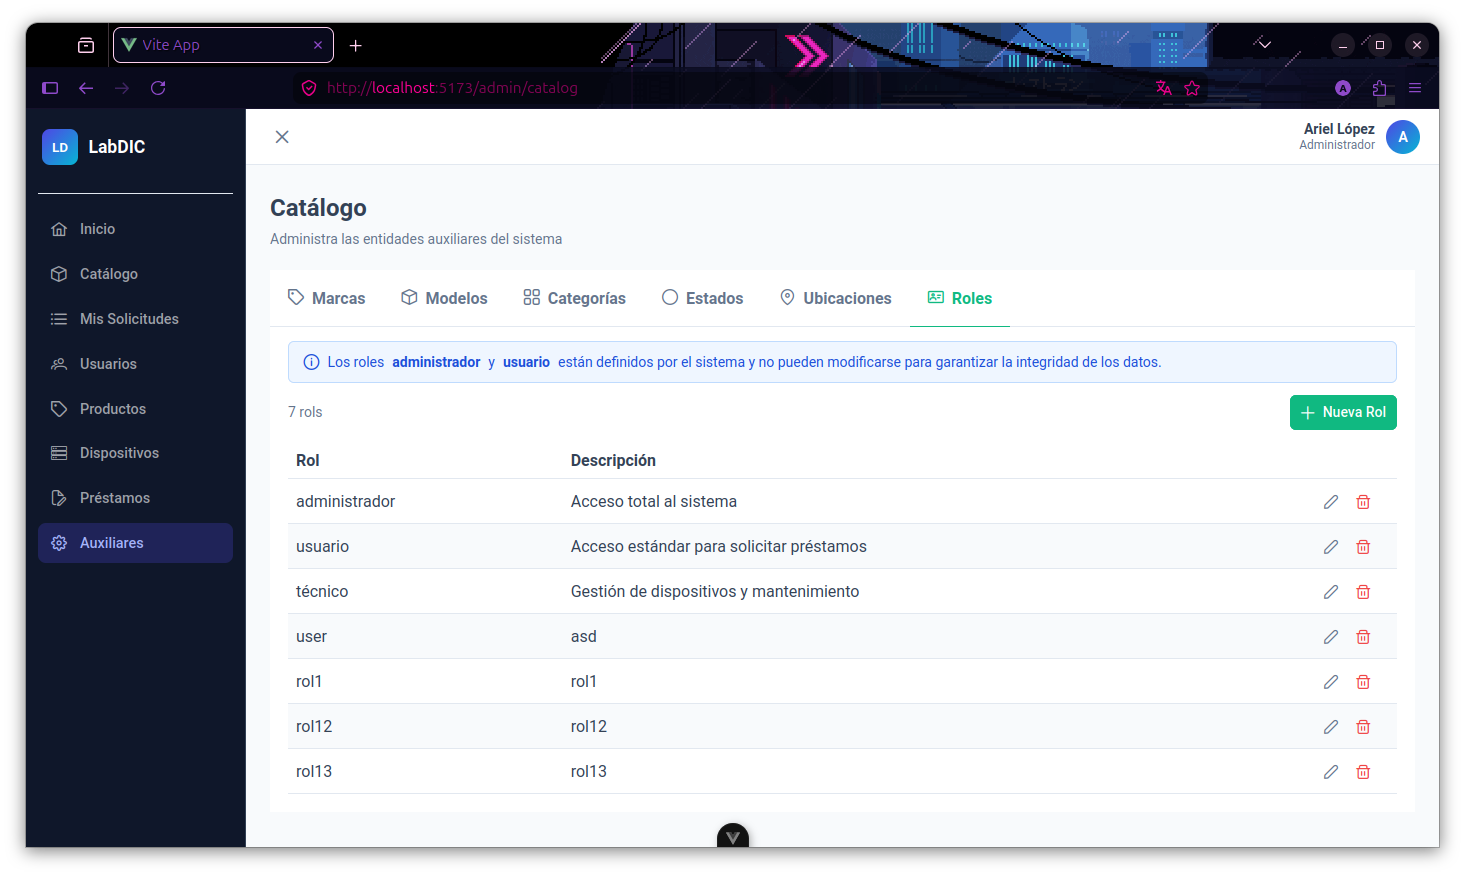
\includegraphics[width=1\textwidth]{img/06_CatalogView_roles.png}
	\caption{Vista de catálogo — sección de roles}
	\label{fig:06_catalog_roles}
\end{figure}
\begin{figure}[H]
	\centering
	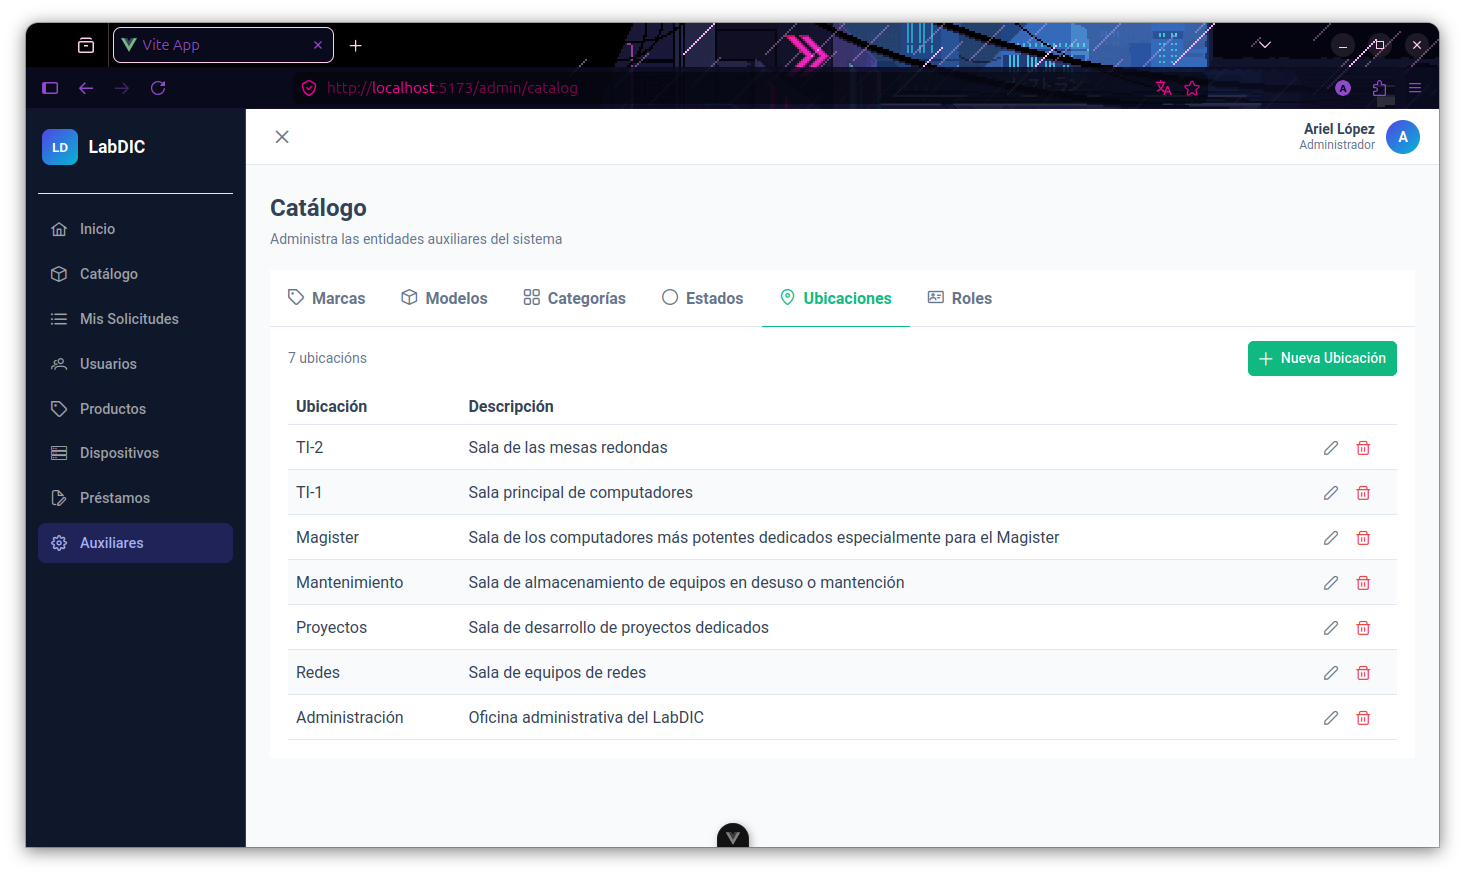
\includegraphics[width=1\textwidth]{img/07_CatalogView_ubicaciones.png}
	\caption{Vista de catálogo — sección de ubicaciones}
	\label{fig:07_catalog_ubicaciones}
\end{figure}
\begin{figure}[H]
	\centering
	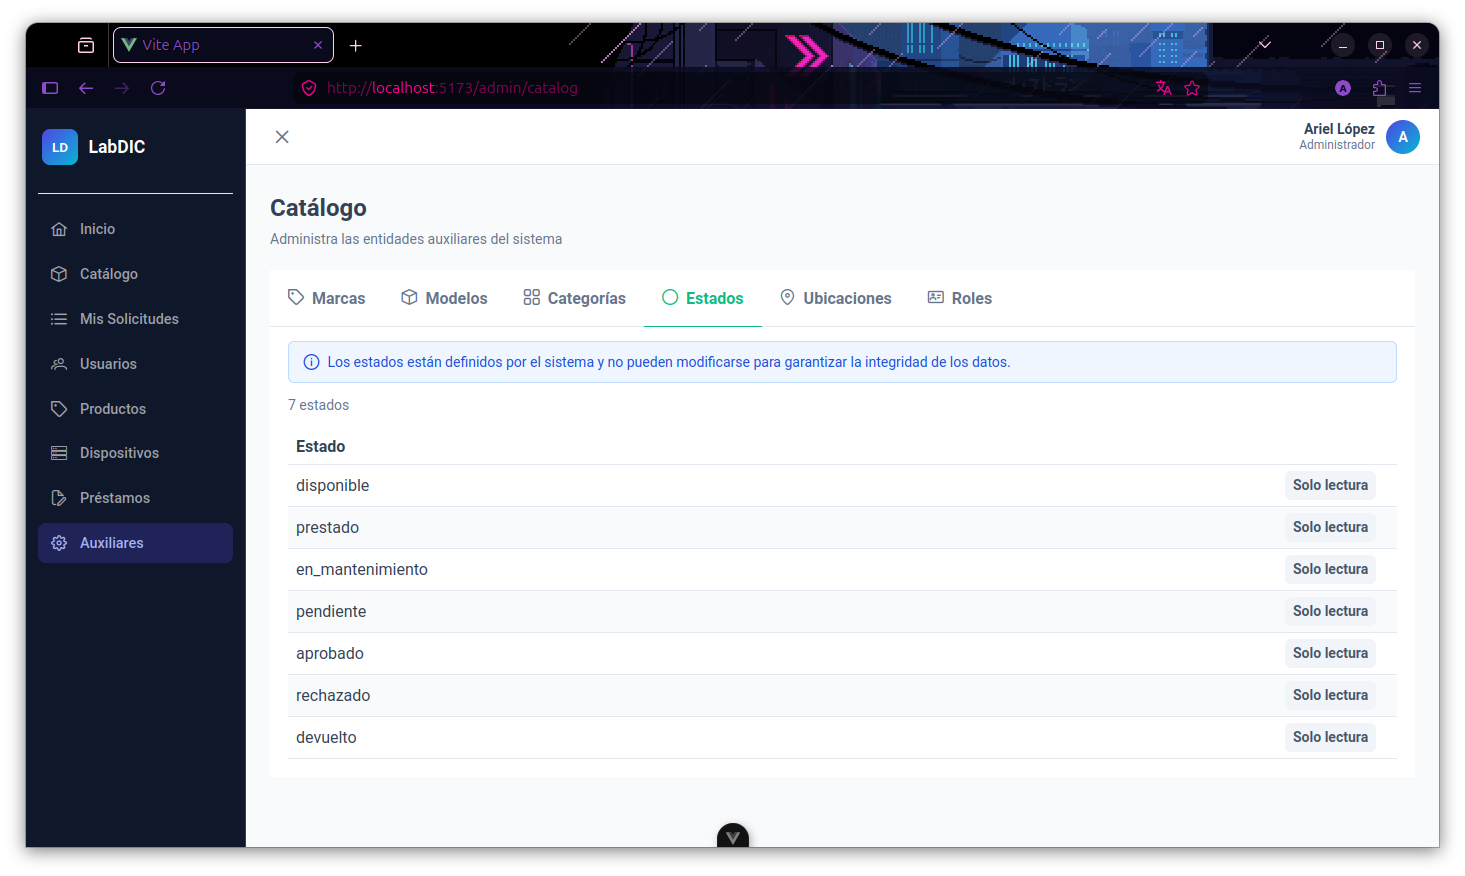
\includegraphics[width=1\textwidth]{img/08_CatalogView_estados.png}
	\caption{Vista de catálogo — sección de estados}
	\label{fig:08_catalog_estados}
\end{figure}
\begin{figure}[H]
	\centering
	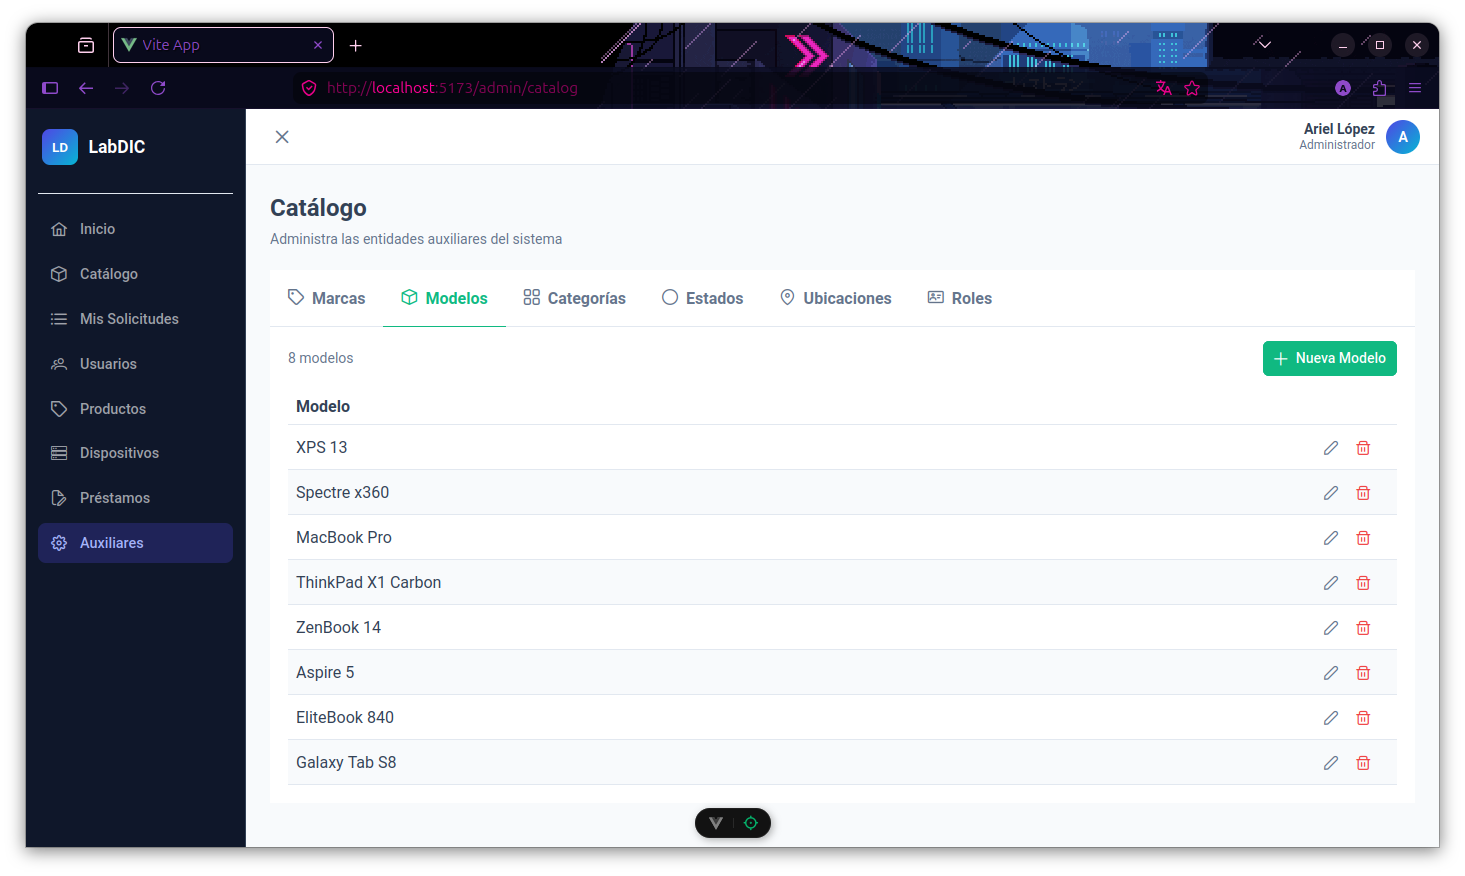
\includegraphics[width=1\textwidth]{img/09_CatalogView_modelos.png}
	\caption{Vista de catálogo — sección de modelos}
	\label{fig:09_catalog_modelos}
\end{figure}
\begin{figure}[H]
	\centering
	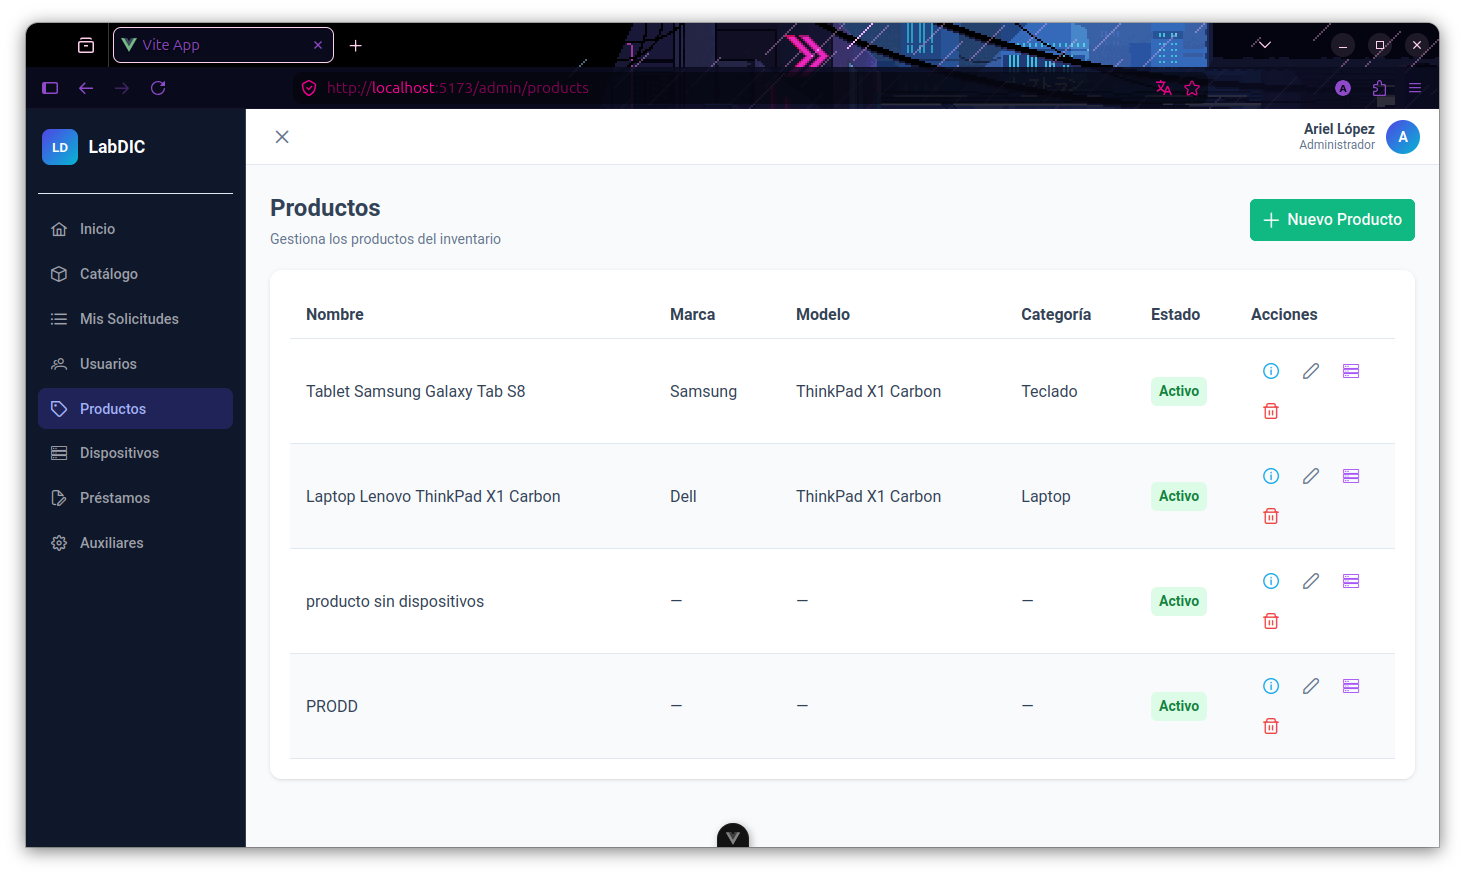
\includegraphics[width=1\textwidth]{img/10_ProductsListView_admin.png}
	\caption{Vista de administración de productos}
	\label{fig:10_products_list_admin}
\end{figure}
\begin{figure}[H]
	\centering
	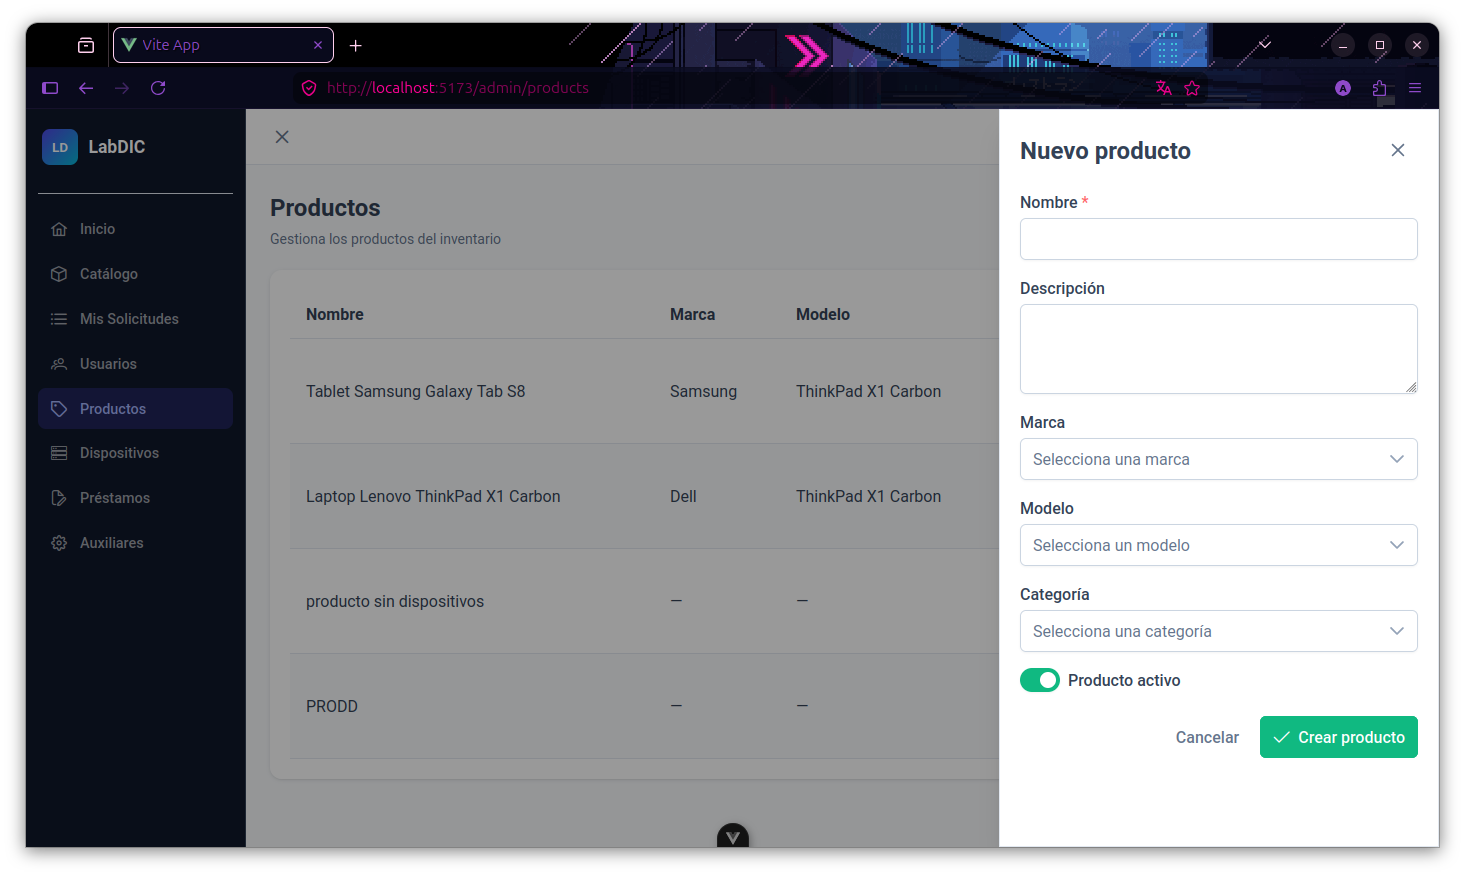
\includegraphics[width=1\textwidth]{img/11_ProductsListView_admin_nuevo_producto.png}
	\caption{Vista de administración de productos — formulario de nuevo producto}
	\label{fig:11_products_list_nuevo}
\end{figure}
\begin{figure}[H]
	\centering
	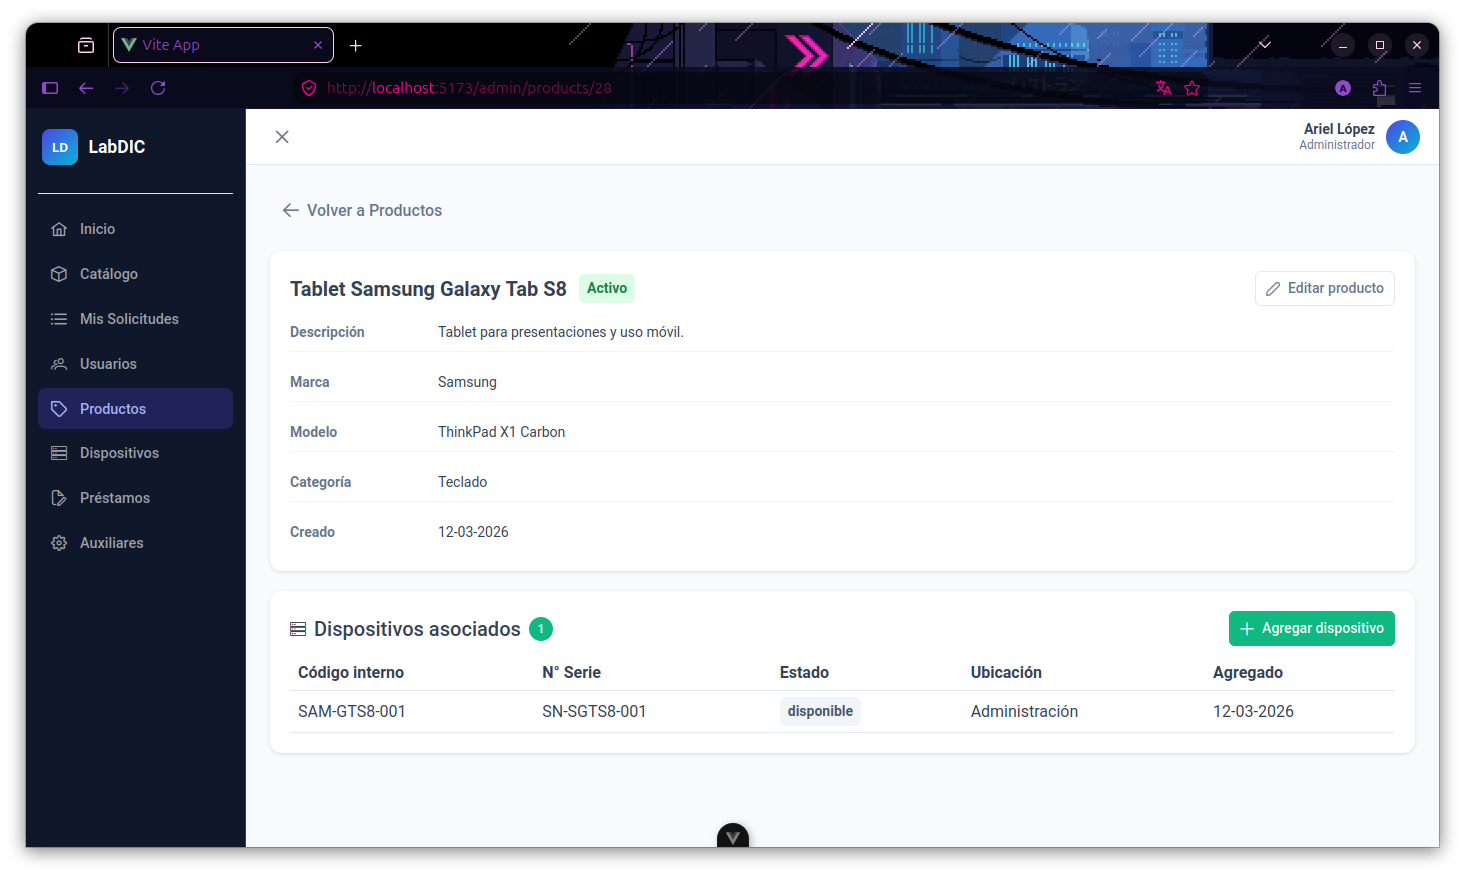
\includegraphics[width=1\textwidth]{img/12_ProductsListView_admin_detalles.png}
	\caption{Vista de administración de productos — detalle de producto}
	\label{fig:12_products_list_detalles}
\end{figure}
\begin{figure}[H]
	\centering
	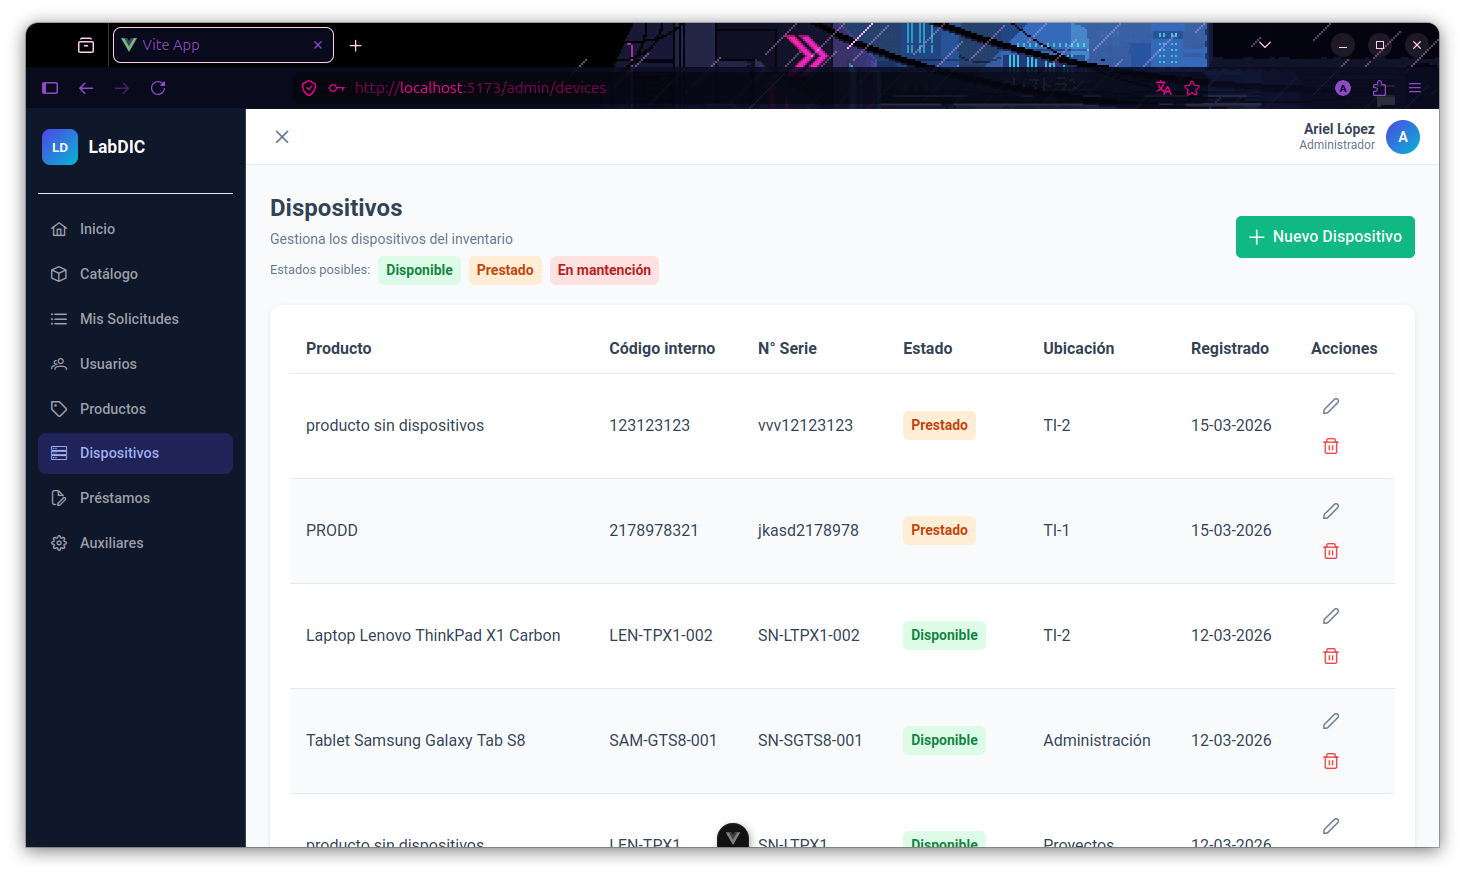
\includegraphics[width=1\textwidth]{img/13_DevicesListView.png}
	\caption{Vista de administración de dispositivos}
	\label{fig:13_devices_list_view}
\end{figure}
\begin{figure}[H]
	\centering
	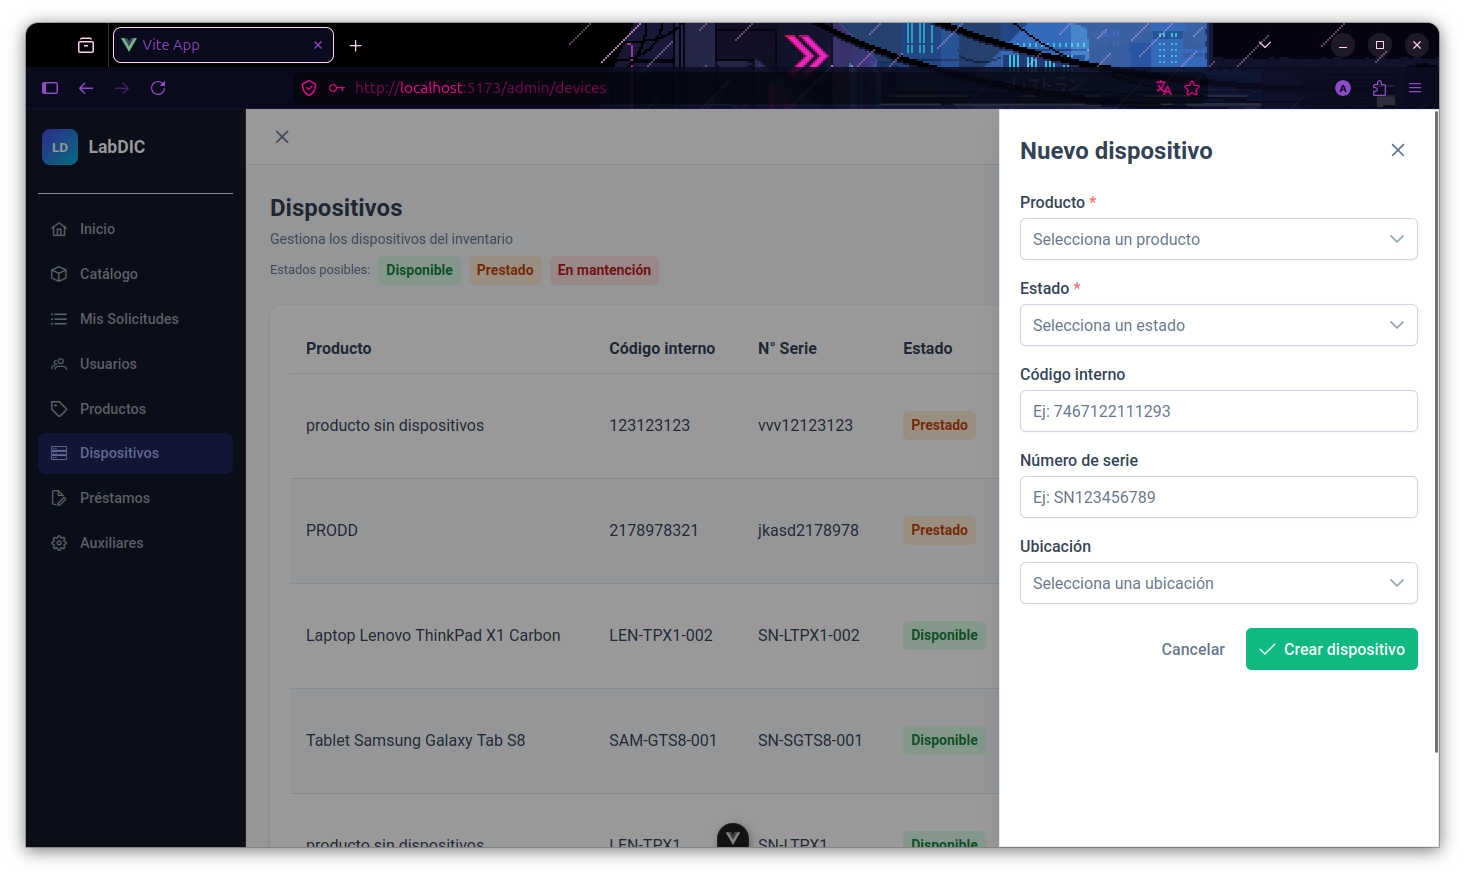
\includegraphics[width=1\textwidth]{img/14_DevicesListView_agregar.png}
	\caption{Vista de administración de dispositivos — formulario de nuevo dispositivo}
	\label{fig:14_devices_list_agregar}
\end{figure}
\begin{figure}[H]
	\centering
	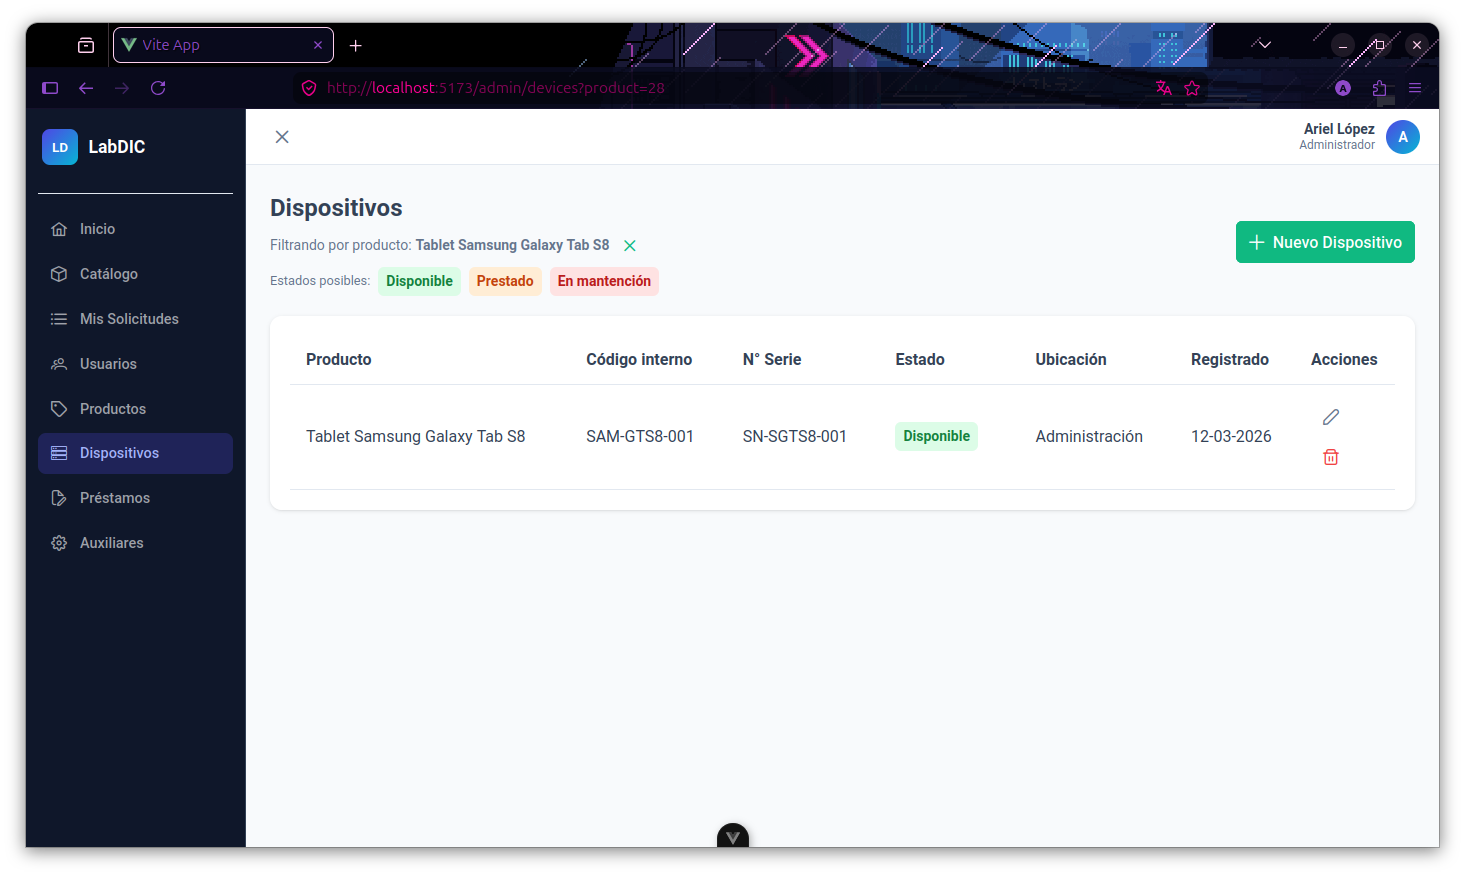
\includegraphics[width=1\textwidth]{img/15_ProductsListView_filtro_DevicesListView.png}
	\caption{Vista de dispositivos filtrada desde detalle de producto}
	\label{fig:15_products_filtro_devices}
\end{figure}
\begin{figure}[H]
	\centering
	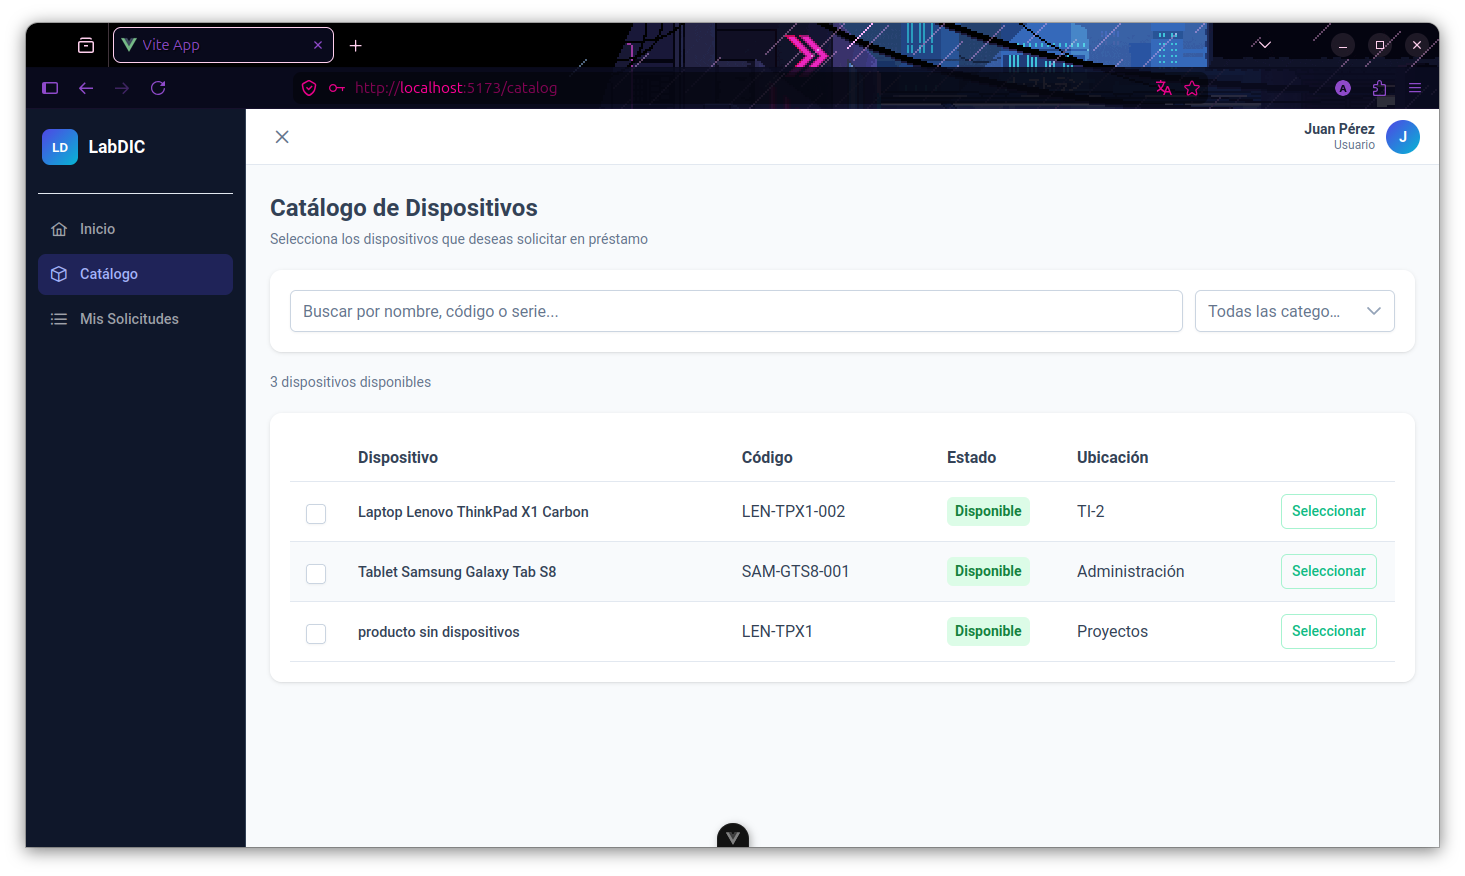
\includegraphics[width=1\textwidth]{img/16_DeviceCatalogView.png}
	\caption{Vista de catálogo de dispositivos disponibles para usuarios}
	\label{fig:16_device_catalog_view}
\end{figure}
\begin{figure}[H]
	\centering
	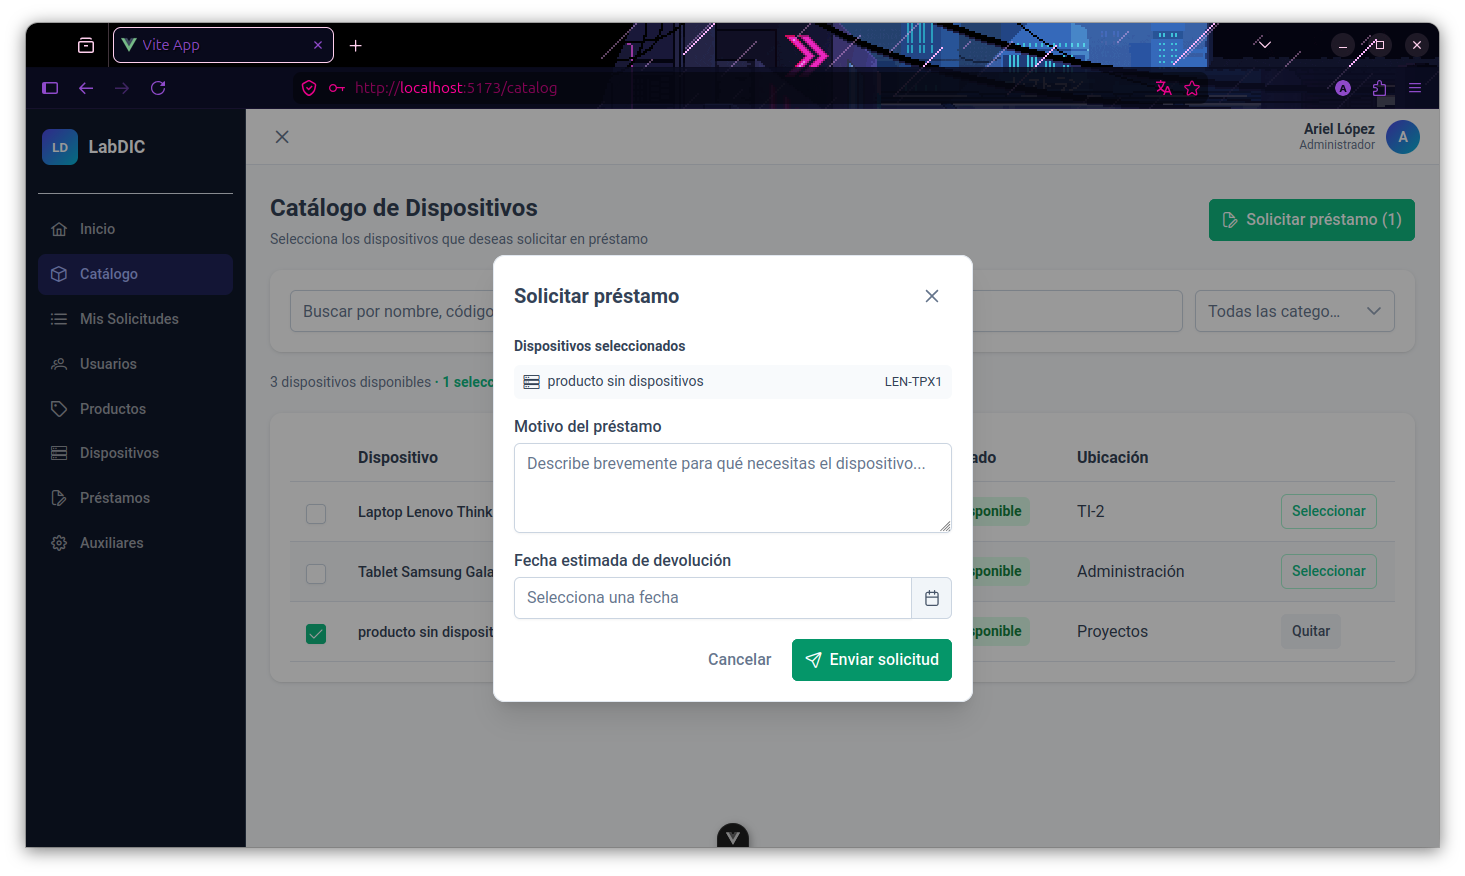
\includegraphics[width=1\textwidth]{img/17_DeviceCatalogView_prestamo.png}
	\caption{Vista de catálogo de dispositivos — formulario de solicitud de préstamo}
	\label{fig:17_device_catalog_prestamo}
\end{figure}
\begin{figure}[H]
	\centering
	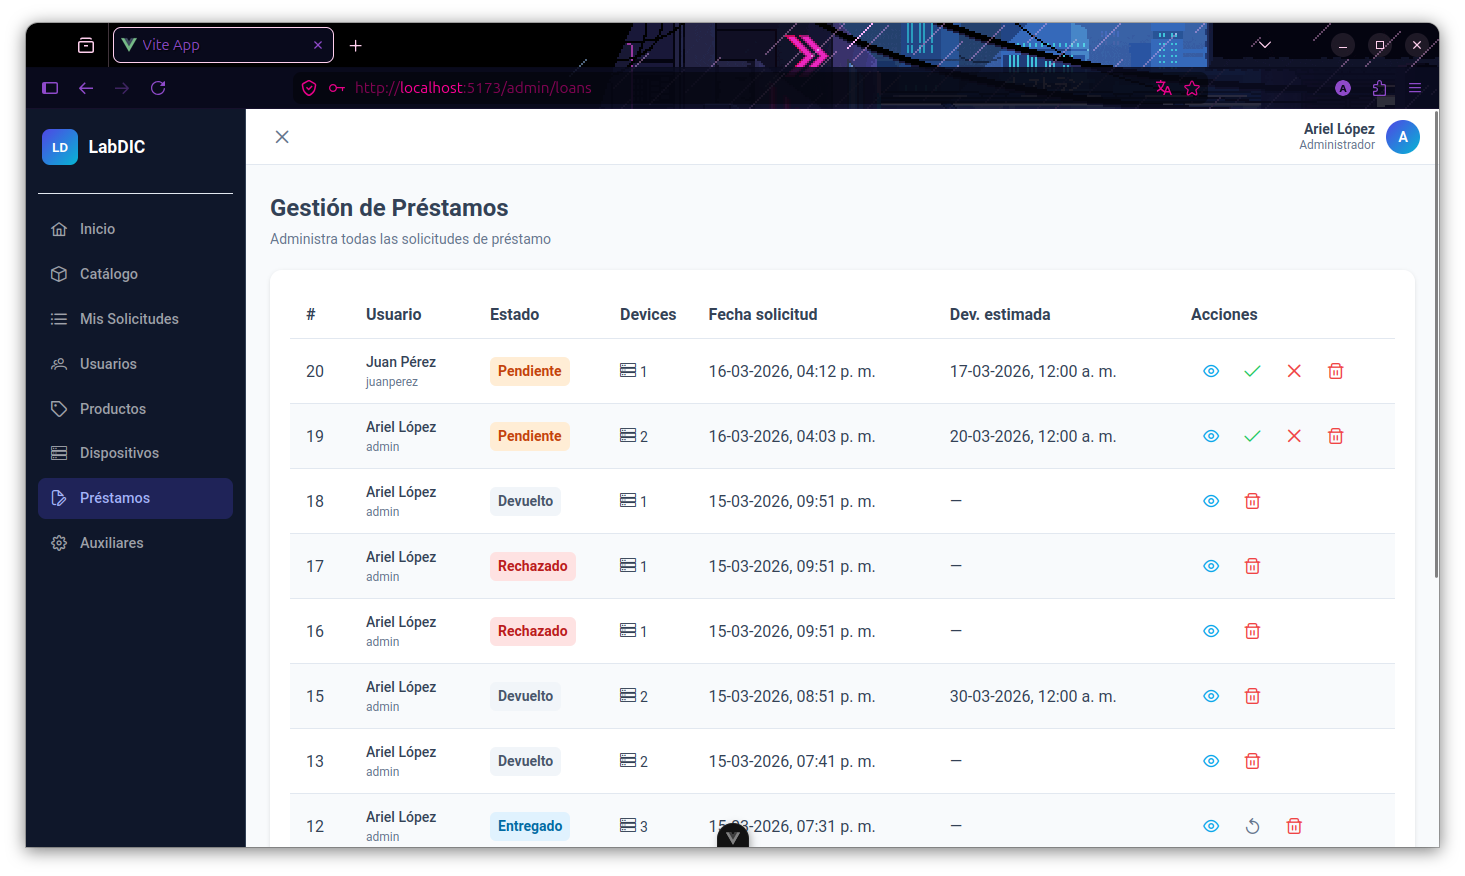
\includegraphics[width=1\textwidth]{img/18_AdminLoansView.png}
	\caption{Vista de administración de solicitudes de préstamo}
	\label{fig:18_admin_loans_view}
\end{figure}
\begin{figure}[H]
	\centering
	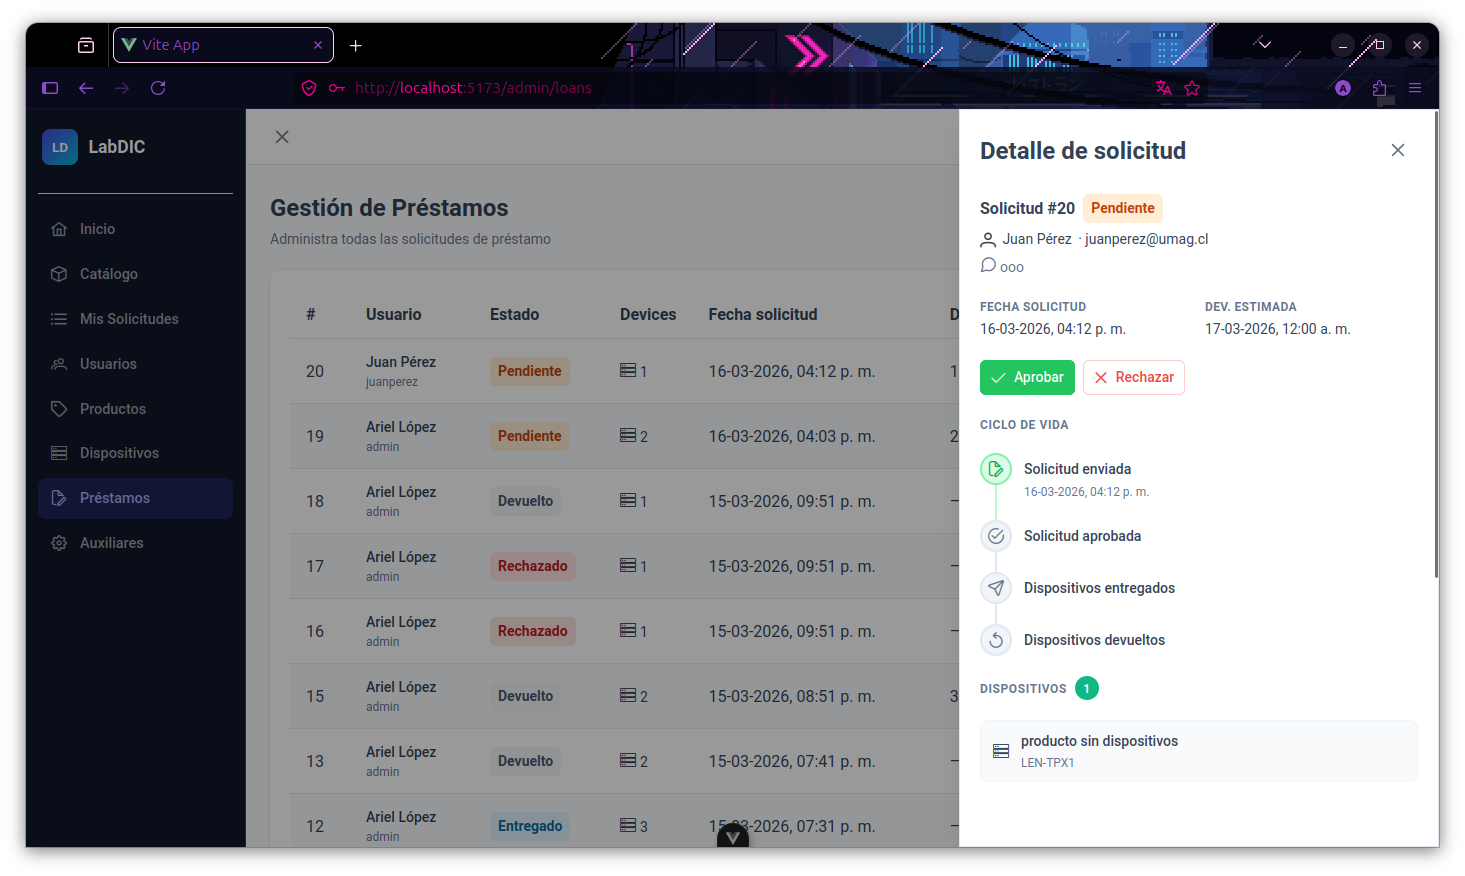
\includegraphics[width=1\textwidth]{img/19_AdminLoansView_ciclo_inicial.png}
	\caption{Vista de administración de préstamos — ciclo de vida en estado inicial}
	\label{fig:19_admin_loans_ciclo_inicial}
\end{figure}
\begin{figure}[H]
	\centering
	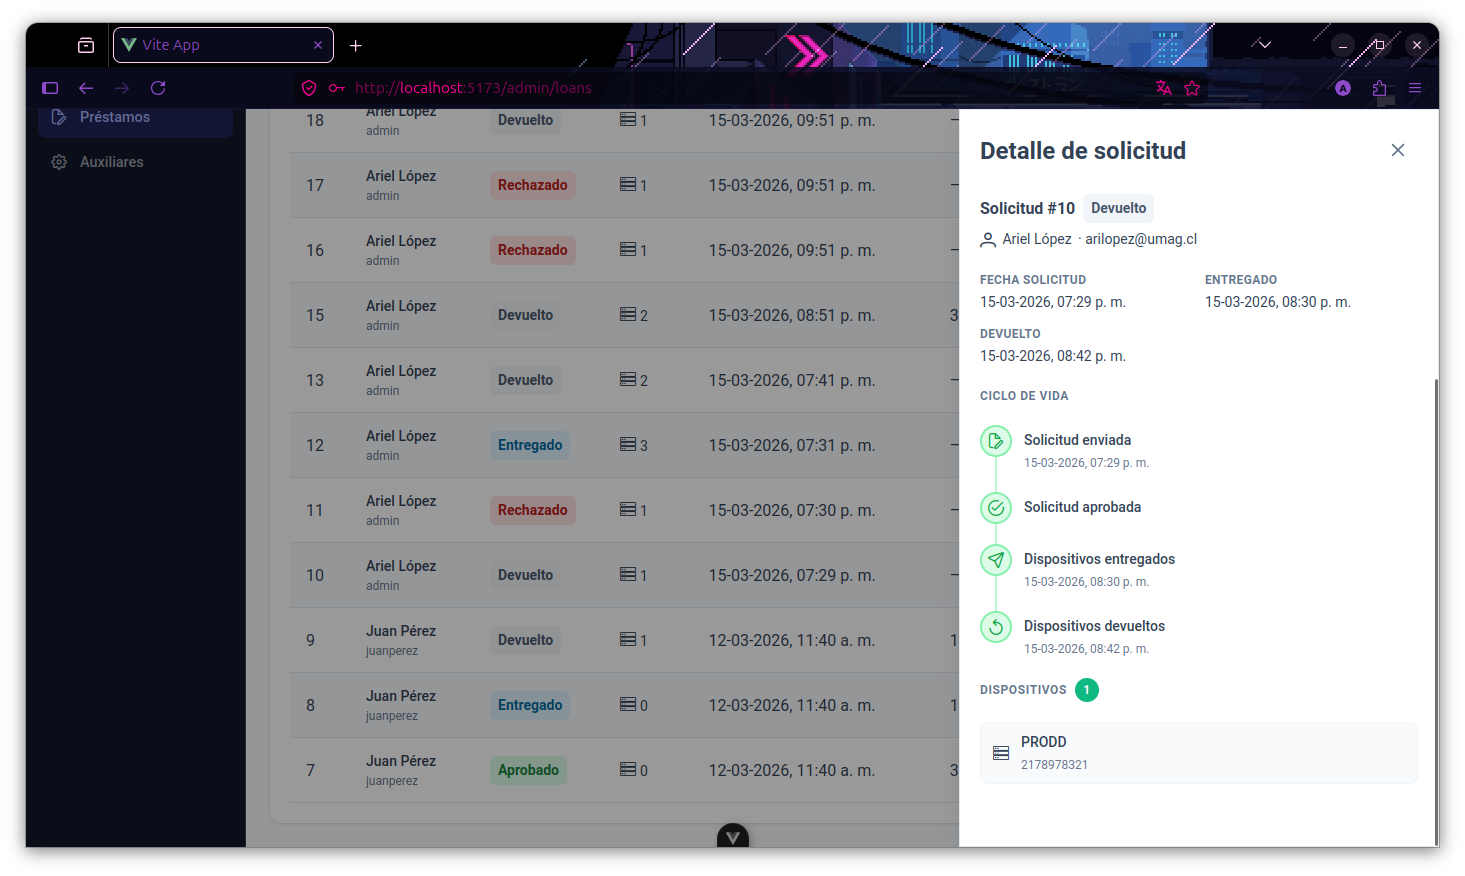
\includegraphics[width=1\textwidth]{img/20_AdminLoansView_ciclo_finalizado.png}
	\caption{Vista de administración de préstamos — ciclo de vida finalizado}
	\label{fig:20_admin_loans_ciclo_finalizado}
\end{figure}
\begin{figure}[H]
	\centering
	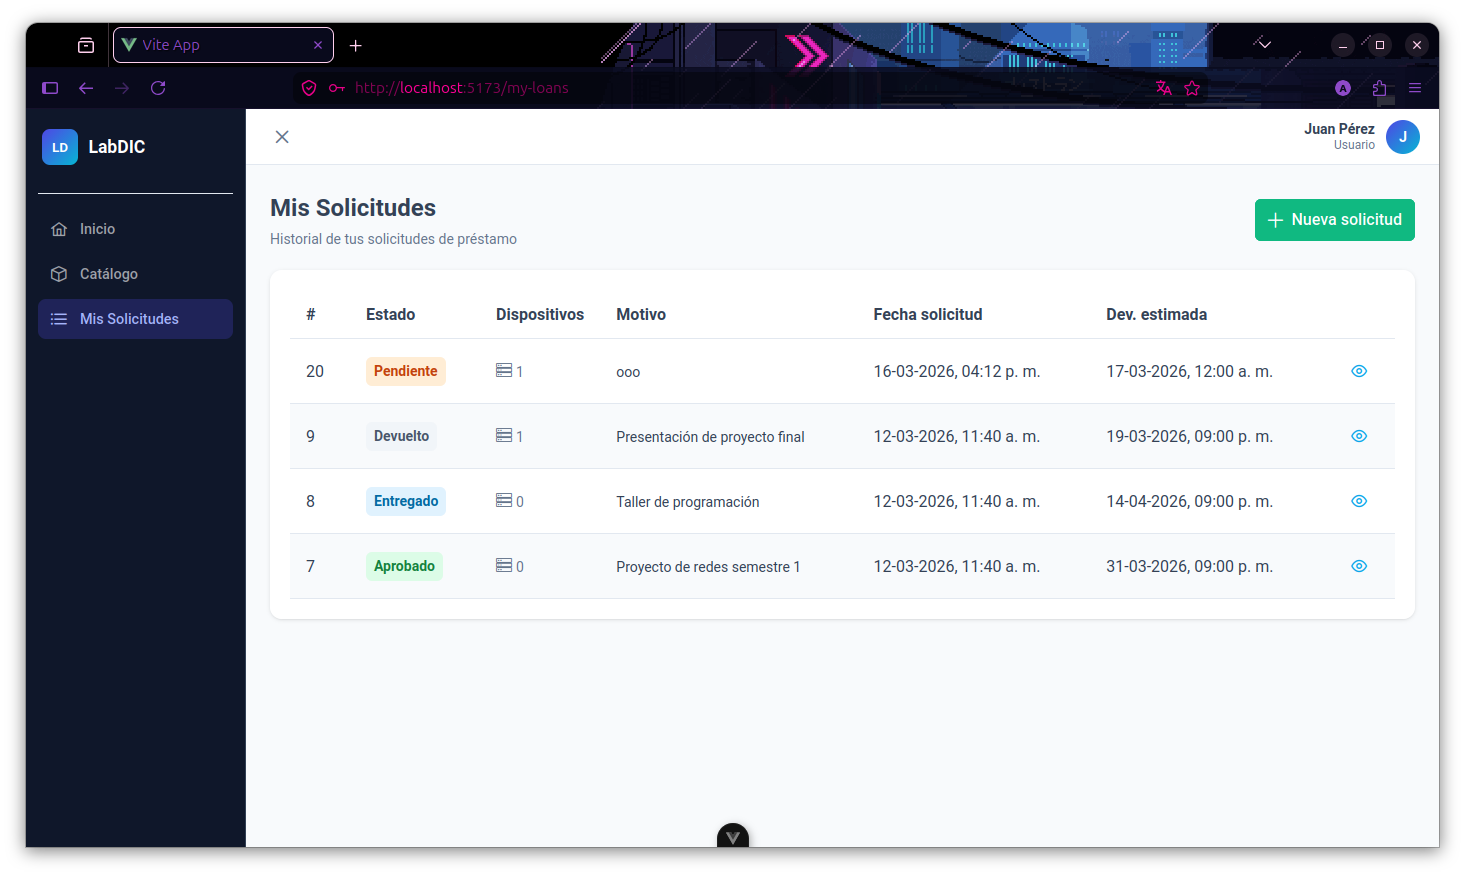
\includegraphics[width=1\textwidth]{img/21_MyLoansView.png}
	\caption{Vista de solicitudes del usuario autenticado}
	\label{fig:21_my_loans_view}
\end{figure}
\begin{figure}[H]
	\centering
	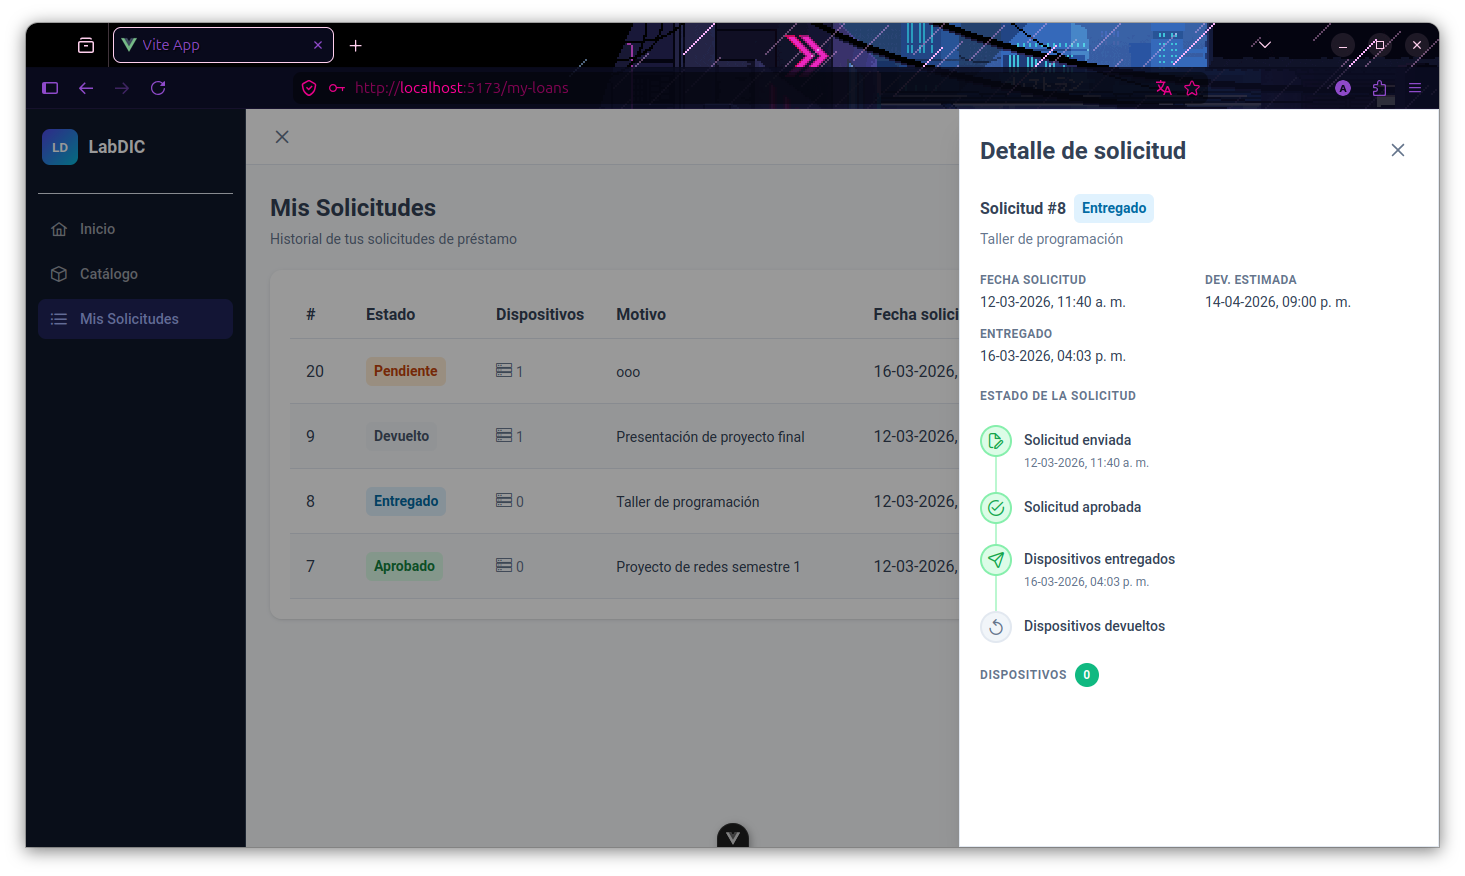
\includegraphics[width=1\textwidth]{img/22_MyLoansView_detalles.png}
	\caption{Vista de solicitudes del usuario autenticado — detalle de solicitud}
	\label{fig:22_my_loans_detalles}
\end{figure}